% Options for packages loaded elsewhere
% Options for packages loaded elsewhere
\PassOptionsToPackage{unicode}{hyperref}
\PassOptionsToPackage{hyphens}{url}
\PassOptionsToPackage{dvipsnames,svgnames,x11names}{xcolor}
%
\documentclass[
  letterpaper,
  DIV=11,
  numbers=noendperiod]{scrreprt}
\usepackage{xcolor}
\usepackage{amsmath,amssymb}
\setcounter{secnumdepth}{5}
\usepackage{iftex}
\ifPDFTeX
  \usepackage[T1]{fontenc}
  \usepackage[utf8]{inputenc}
  \usepackage{textcomp} % provide euro and other symbols
\else % if luatex or xetex
  \usepackage{unicode-math} % this also loads fontspec
  \defaultfontfeatures{Scale=MatchLowercase}
  \defaultfontfeatures[\rmfamily]{Ligatures=TeX,Scale=1}
\fi
\usepackage{lmodern}
\ifPDFTeX\else
  % xetex/luatex font selection
\fi
% Use upquote if available, for straight quotes in verbatim environments
\IfFileExists{upquote.sty}{\usepackage{upquote}}{}
\IfFileExists{microtype.sty}{% use microtype if available
  \usepackage[]{microtype}
  \UseMicrotypeSet[protrusion]{basicmath} % disable protrusion for tt fonts
}{}
\makeatletter
\@ifundefined{KOMAClassName}{% if non-KOMA class
  \IfFileExists{parskip.sty}{%
    \usepackage{parskip}
  }{% else
    \setlength{\parindent}{0pt}
    \setlength{\parskip}{6pt plus 2pt minus 1pt}}
}{% if KOMA class
  \KOMAoptions{parskip=half}}
\makeatother
% Make \paragraph and \subparagraph free-standing
\makeatletter
\ifx\paragraph\undefined\else
  \let\oldparagraph\paragraph
  \renewcommand{\paragraph}{
    \@ifstar
      \xxxParagraphStar
      \xxxParagraphNoStar
  }
  \newcommand{\xxxParagraphStar}[1]{\oldparagraph*{#1}\mbox{}}
  \newcommand{\xxxParagraphNoStar}[1]{\oldparagraph{#1}\mbox{}}
\fi
\ifx\subparagraph\undefined\else
  \let\oldsubparagraph\subparagraph
  \renewcommand{\subparagraph}{
    \@ifstar
      \xxxSubParagraphStar
      \xxxSubParagraphNoStar
  }
  \newcommand{\xxxSubParagraphStar}[1]{\oldsubparagraph*{#1}\mbox{}}
  \newcommand{\xxxSubParagraphNoStar}[1]{\oldsubparagraph{#1}\mbox{}}
\fi
\makeatother

\usepackage{color}
\usepackage{fancyvrb}
\newcommand{\VerbBar}{|}
\newcommand{\VERB}{\Verb[commandchars=\\\{\}]}
\DefineVerbatimEnvironment{Highlighting}{Verbatim}{commandchars=\\\{\}}
% Add ',fontsize=\small' for more characters per line
\usepackage{framed}
\definecolor{shadecolor}{RGB}{241,243,245}
\newenvironment{Shaded}{\begin{snugshade}}{\end{snugshade}}
\newcommand{\AlertTok}[1]{\textcolor[rgb]{0.68,0.00,0.00}{#1}}
\newcommand{\AnnotationTok}[1]{\textcolor[rgb]{0.37,0.37,0.37}{#1}}
\newcommand{\AttributeTok}[1]{\textcolor[rgb]{0.40,0.45,0.13}{#1}}
\newcommand{\BaseNTok}[1]{\textcolor[rgb]{0.68,0.00,0.00}{#1}}
\newcommand{\BuiltInTok}[1]{\textcolor[rgb]{0.00,0.23,0.31}{#1}}
\newcommand{\CharTok}[1]{\textcolor[rgb]{0.13,0.47,0.30}{#1}}
\newcommand{\CommentTok}[1]{\textcolor[rgb]{0.37,0.37,0.37}{#1}}
\newcommand{\CommentVarTok}[1]{\textcolor[rgb]{0.37,0.37,0.37}{\textit{#1}}}
\newcommand{\ConstantTok}[1]{\textcolor[rgb]{0.56,0.35,0.01}{#1}}
\newcommand{\ControlFlowTok}[1]{\textcolor[rgb]{0.00,0.23,0.31}{\textbf{#1}}}
\newcommand{\DataTypeTok}[1]{\textcolor[rgb]{0.68,0.00,0.00}{#1}}
\newcommand{\DecValTok}[1]{\textcolor[rgb]{0.68,0.00,0.00}{#1}}
\newcommand{\DocumentationTok}[1]{\textcolor[rgb]{0.37,0.37,0.37}{\textit{#1}}}
\newcommand{\ErrorTok}[1]{\textcolor[rgb]{0.68,0.00,0.00}{#1}}
\newcommand{\ExtensionTok}[1]{\textcolor[rgb]{0.00,0.23,0.31}{#1}}
\newcommand{\FloatTok}[1]{\textcolor[rgb]{0.68,0.00,0.00}{#1}}
\newcommand{\FunctionTok}[1]{\textcolor[rgb]{0.28,0.35,0.67}{#1}}
\newcommand{\ImportTok}[1]{\textcolor[rgb]{0.00,0.46,0.62}{#1}}
\newcommand{\InformationTok}[1]{\textcolor[rgb]{0.37,0.37,0.37}{#1}}
\newcommand{\KeywordTok}[1]{\textcolor[rgb]{0.00,0.23,0.31}{\textbf{#1}}}
\newcommand{\NormalTok}[1]{\textcolor[rgb]{0.00,0.23,0.31}{#1}}
\newcommand{\OperatorTok}[1]{\textcolor[rgb]{0.37,0.37,0.37}{#1}}
\newcommand{\OtherTok}[1]{\textcolor[rgb]{0.00,0.23,0.31}{#1}}
\newcommand{\PreprocessorTok}[1]{\textcolor[rgb]{0.68,0.00,0.00}{#1}}
\newcommand{\RegionMarkerTok}[1]{\textcolor[rgb]{0.00,0.23,0.31}{#1}}
\newcommand{\SpecialCharTok}[1]{\textcolor[rgb]{0.37,0.37,0.37}{#1}}
\newcommand{\SpecialStringTok}[1]{\textcolor[rgb]{0.13,0.47,0.30}{#1}}
\newcommand{\StringTok}[1]{\textcolor[rgb]{0.13,0.47,0.30}{#1}}
\newcommand{\VariableTok}[1]{\textcolor[rgb]{0.07,0.07,0.07}{#1}}
\newcommand{\VerbatimStringTok}[1]{\textcolor[rgb]{0.13,0.47,0.30}{#1}}
\newcommand{\WarningTok}[1]{\textcolor[rgb]{0.37,0.37,0.37}{\textit{#1}}}

\usepackage{longtable,booktabs,array}
\usepackage{calc} % for calculating minipage widths
% Correct order of tables after \paragraph or \subparagraph
\usepackage{etoolbox}
\makeatletter
\patchcmd\longtable{\par}{\if@noskipsec\mbox{}\fi\par}{}{}
\makeatother
% Allow footnotes in longtable head/foot
\IfFileExists{footnotehyper.sty}{\usepackage{footnotehyper}}{\usepackage{footnote}}
\makesavenoteenv{longtable}
\usepackage{graphicx}
\makeatletter
\newsavebox\pandoc@box
\newcommand*\pandocbounded[1]{% scales image to fit in text height/width
  \sbox\pandoc@box{#1}%
  \Gscale@div\@tempa{\textheight}{\dimexpr\ht\pandoc@box+\dp\pandoc@box\relax}%
  \Gscale@div\@tempb{\linewidth}{\wd\pandoc@box}%
  \ifdim\@tempb\p@<\@tempa\p@\let\@tempa\@tempb\fi% select the smaller of both
  \ifdim\@tempa\p@<\p@\scalebox{\@tempa}{\usebox\pandoc@box}%
  \else\usebox{\pandoc@box}%
  \fi%
}
% Set default figure placement to htbp
\def\fps@figure{htbp}
\makeatother


% definitions for citeproc citations
\NewDocumentCommand\citeproctext{}{}
\NewDocumentCommand\citeproc{mm}{%
  \begingroup\def\citeproctext{#2}\cite{#1}\endgroup}
\makeatletter
 % allow citations to break across lines
 \let\@cite@ofmt\@firstofone
 % avoid brackets around text for \cite:
 \def\@biblabel#1{}
 \def\@cite#1#2{{#1\if@tempswa , #2\fi}}
\makeatother
\newlength{\cslhangindent}
\setlength{\cslhangindent}{1.5em}
\newlength{\csllabelwidth}
\setlength{\csllabelwidth}{3em}
\newenvironment{CSLReferences}[2] % #1 hanging-indent, #2 entry-spacing
 {\begin{list}{}{%
  \setlength{\itemindent}{0pt}
  \setlength{\leftmargin}{0pt}
  \setlength{\parsep}{0pt}
  % turn on hanging indent if param 1 is 1
  \ifodd #1
   \setlength{\leftmargin}{\cslhangindent}
   \setlength{\itemindent}{-1\cslhangindent}
  \fi
  % set entry spacing
  \setlength{\itemsep}{#2\baselineskip}}}
 {\end{list}}
\usepackage{calc}
\newcommand{\CSLBlock}[1]{\hfill\break\parbox[t]{\linewidth}{\strut\ignorespaces#1\strut}}
\newcommand{\CSLLeftMargin}[1]{\parbox[t]{\csllabelwidth}{\strut#1\strut}}
\newcommand{\CSLRightInline}[1]{\parbox[t]{\linewidth - \csllabelwidth}{\strut#1\strut}}
\newcommand{\CSLIndent}[1]{\hspace{\cslhangindent}#1}



\setlength{\emergencystretch}{3em} % prevent overfull lines

\providecommand{\tightlist}{%
  \setlength{\itemsep}{0pt}\setlength{\parskip}{0pt}}



 


\KOMAoption{captions}{tableheading}
\makeatletter
\@ifpackageloaded{tcolorbox}{}{\usepackage[skins,breakable]{tcolorbox}}
\@ifpackageloaded{fontawesome5}{}{\usepackage{fontawesome5}}
\definecolor{quarto-callout-color}{HTML}{909090}
\definecolor{quarto-callout-note-color}{HTML}{0758E5}
\definecolor{quarto-callout-important-color}{HTML}{CC1914}
\definecolor{quarto-callout-warning-color}{HTML}{EB9113}
\definecolor{quarto-callout-tip-color}{HTML}{00A047}
\definecolor{quarto-callout-caution-color}{HTML}{FC5300}
\definecolor{quarto-callout-color-frame}{HTML}{acacac}
\definecolor{quarto-callout-note-color-frame}{HTML}{4582ec}
\definecolor{quarto-callout-important-color-frame}{HTML}{d9534f}
\definecolor{quarto-callout-warning-color-frame}{HTML}{f0ad4e}
\definecolor{quarto-callout-tip-color-frame}{HTML}{02b875}
\definecolor{quarto-callout-caution-color-frame}{HTML}{fd7e14}
\makeatother
\makeatletter
\@ifpackageloaded{bookmark}{}{\usepackage{bookmark}}
\makeatother
\makeatletter
\@ifpackageloaded{caption}{}{\usepackage{caption}}
\AtBeginDocument{%
\ifdefined\contentsname
  \renewcommand*\contentsname{Table of contents}
\else
  \newcommand\contentsname{Table of contents}
\fi
\ifdefined\listfigurename
  \renewcommand*\listfigurename{List of Figures}
\else
  \newcommand\listfigurename{List of Figures}
\fi
\ifdefined\listtablename
  \renewcommand*\listtablename{List of Tables}
\else
  \newcommand\listtablename{List of Tables}
\fi
\ifdefined\figurename
  \renewcommand*\figurename{Figure}
\else
  \newcommand\figurename{Figure}
\fi
\ifdefined\tablename
  \renewcommand*\tablename{Table}
\else
  \newcommand\tablename{Table}
\fi
}
\@ifpackageloaded{float}{}{\usepackage{float}}
\floatstyle{ruled}
\@ifundefined{c@chapter}{\newfloat{codelisting}{h}{lop}}{\newfloat{codelisting}{h}{lop}[chapter]}
\floatname{codelisting}{Listing}
\newcommand*\listoflistings{\listof{codelisting}{List of Listings}}
\makeatother
\makeatletter
\makeatother
\makeatletter
\@ifpackageloaded{caption}{}{\usepackage{caption}}
\@ifpackageloaded{subcaption}{}{\usepackage{subcaption}}
\makeatother
\usepackage{bookmark}
\IfFileExists{xurl.sty}{\usepackage{xurl}}{} % add URL line breaks if available
\urlstyle{same}
\hypersetup{
  pdftitle={Using Hidden Markov Models for Animal Tracking},
  pdfauthor={Collin Henkel},
  colorlinks=true,
  linkcolor={blue},
  filecolor={Maroon},
  citecolor={Blue},
  urlcolor={Blue},
  pdfcreator={LaTeX via pandoc}}


\title{Using Hidden Markov Models for Animal Tracking}
\author{Collin Henkel}
\date{March 6, 2026}
\begin{document}
\maketitle

\renewcommand*\contentsname{Table of contents}
{
\hypersetup{linkcolor=}
\setcounter{tocdepth}{2}
\tableofcontents
}

\bookmarksetup{startatroot}

\chapter*{Assignment Flow}\label{assignment-flow}
\addcontentsline{toc}{chapter}{Assignment Flow}

\markboth{Assignment Flow}{Assignment Flow}

This project is set up to scaffold this user guide and set you up for
success.

Start at \texttt{topic.qmd} and identify a topic for your user guide.

Once you've proposed a topic and received my approval/feedback, you can
convert the contents of \texttt{topic.qmd} into an introductory
paragraph in your report. Please leave the \texttt{topic.qmd} file as an
appendix, to document the different stages of this project.

Once we've agreed on a topic for your user guide, you will proceed to
\texttt{needs.qmd} and \texttt{task-analysis.qmd}. Both will be
submitted at the same check-in, and both will be included in your final
report as appendices. You should be able to re-purpose most of the
information in \texttt{task-analysis.qmd} to orient the user to
different components of the task you've chosen.

Your next step is to actually write the content that satisfies the work
you outlined in \texttt{task-analysis.qmd}.

Once you're finished with that, ideally, you'll have plenty of time to
edit and streamline your report. Feel free to trade reports with a
friend and try to complete your friend's task - this will help you both
identify areas where the guide isn't as clear. Try to complete the task
with a different data set - that often helps find trouble spots.

When you submit your final report, you may remove \texttt{index.qmd}
from the \texttt{\_quarto.yml} file, which will remove this chapter
(which is quite unnecessary for your user) from the report. You should
also take the time to make sure your name is listed as both author and
copyright holder in the \texttt{\_quarto.yml} file. Feel free to make a
custom cover for your manual if you would like to do so. You can also
tweak the CSS/theme for the book, so long as you're conscious of
accessibility concerns.

\begin{tcolorbox}[enhanced jigsaw, colback=white, colbacktitle=quarto-callout-caution-color!10!white, coltitle=black, opacitybacktitle=0.6, bottomrule=.15mm, colframe=quarto-callout-caution-color-frame, toptitle=1mm, leftrule=.75mm, opacityback=0, bottomtitle=1mm, toprule=.15mm, rightrule=.15mm, titlerule=0mm, breakable, left=2mm, arc=.35mm, title=\textcolor{quarto-callout-caution-color}{\faFire}\hspace{0.5em}{Building the report}]

If you are using RStudio to complete this report, you can hit
(Ctrl/Cmd)-Shift-B to build the whole report. You can also type
\texttt{quarto\ render\ .} on the command line in the project folder to
accomplish the same thing.

If you have questions about how to customize or debug your book, it may
be helpful to start at the quarto book documentation
(\textbf{positpbcCreatingBook2024?}).

\end{tcolorbox}

\bookmarksetup{startatroot}

\chapter{Using Hidden Markov Models for Animal
Tracking}\label{using-hidden-markov-models-for-animal-tracking}

Hidden Markov Models (HMMs) are commonly used to analyze animal movement
data. In many tracking datasets we observe locations over time, but we
do not directly observe the behavior of the animal. HMMs let researchers
infer hidden behavior states like resting, traveling, or foraging based
on movement patterns. This guide explains the basic idea behind fitting
an HMM to tracking data using R and interpreting the results.

\section{Prerequisites}\label{prerequisites}

Before following this guide, users should:

\begin{itemize}
\tightlist
\item
  Have basic knowledge of R and RStudio
\item
  Install the ``moveHMM'' package
\item
  Have tracking data with coordinates and timestamps
\item
  Understand basic statistical concepts such as probability
  distributions
\end{itemize}

\section{Required Data}\label{required-data}

To apply an HMM to movement data, the dataset should include:

\begin{itemize}
\tightlist
\item
  Animal location coordinates (latitude and longitude)
\item
  Timestamps for each observation
\item
  Observations ordered in time
\end{itemize}

From these values we can find:

\begin{itemize}
\tightlist
\item
  \textbf{Step length} (distance between consecutive locations)
\item
  \textbf{Turning angle} (change in movement direction)
\end{itemize}

These variables are commonly used as the observed data in animal
movement HMMs.

\section{Software Setup}\label{software-setup}

There are multiple R packages that can fit HMMs for movement data. One
that is commonly used is the \texttt{moveHMM} package Théo Michelot,
Langrock, and Patterson (2016).

To install and load the package and its dependencies:

\begin{Shaded}
\begin{Highlighting}[]
\FunctionTok{install.packages}\NormalTok{(}\StringTok{"CircStats"}\NormalTok{)}
\FunctionTok{install.packages}\NormalTok{(}\StringTok{"moveHMM"}\NormalTok{)}
\FunctionTok{library}\NormalTok{(moveHMM)}
\end{Highlighting}
\end{Shaded}

We can then load our library and some of its example data:

\begin{Shaded}
\begin{Highlighting}[]
\FunctionTok{library}\NormalTok{(moveHMM)}
\end{Highlighting}
\end{Shaded}

\begin{verbatim}
Warning: package 'moveHMM' was built under R version 4.3.3
\end{verbatim}

\begin{verbatim}
Loading required package: CircStats
\end{verbatim}

\begin{verbatim}
Loading required package: MASS
\end{verbatim}

\begin{verbatim}
Loading required package: boot
\end{verbatim}

\begin{Shaded}
\begin{Highlighting}[]
\FunctionTok{data}\NormalTok{(}\StringTok{"elk\_data"}\NormalTok{)}

\FunctionTok{head}\NormalTok{(elk\_data)}
\end{Highlighting}
\end{Shaded}

\begin{verbatim}
       ID Easting Northing dist_water
1 elk-115  769928  4992847     200.00
2 elk-115  766875  4997444     600.52
3 elk-115  765949  4998516     561.81
4 elk-115  765938  4998277     550.00
5 elk-115  766275  4998005     302.08
6 elk-115  766368  4998051     213.60
\end{verbatim}

\section{Preparing the Data}\label{preparing-the-data}

After loading the data, the \texttt{prepData()} function in the package
can calculate step lengths and turning angles from the data using type =
``UTM'' since we have Easting/Northing data rather than
Latitude/Longitude:

\begin{Shaded}
\begin{Highlighting}[]
\NormalTok{data }\OtherTok{\textless{}{-}} \FunctionTok{prepData}\NormalTok{(elk\_data, }\AttributeTok{type=}\StringTok{"UTM"}\NormalTok{, }\AttributeTok{coordNames=}\FunctionTok{c}\NormalTok{(}\StringTok{"Easting"}\NormalTok{,}\StringTok{"Northing"}\NormalTok{))}
\FunctionTok{plot}\NormalTok{(data,}\AttributeTok{compact=}\NormalTok{T)}
\end{Highlighting}
\end{Shaded}

\pandocbounded{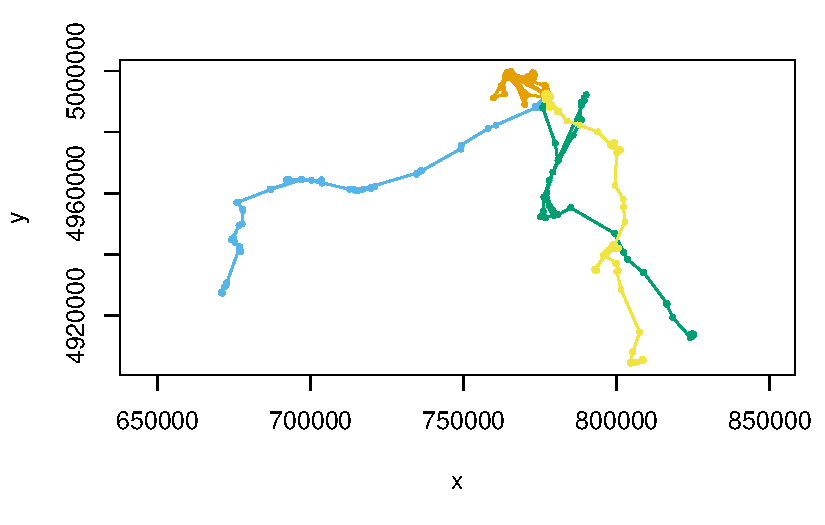
\includegraphics[keepaspectratio]{guide_files/figure-pdf/unnamed-chunk-2-1.pdf}}

\pandocbounded{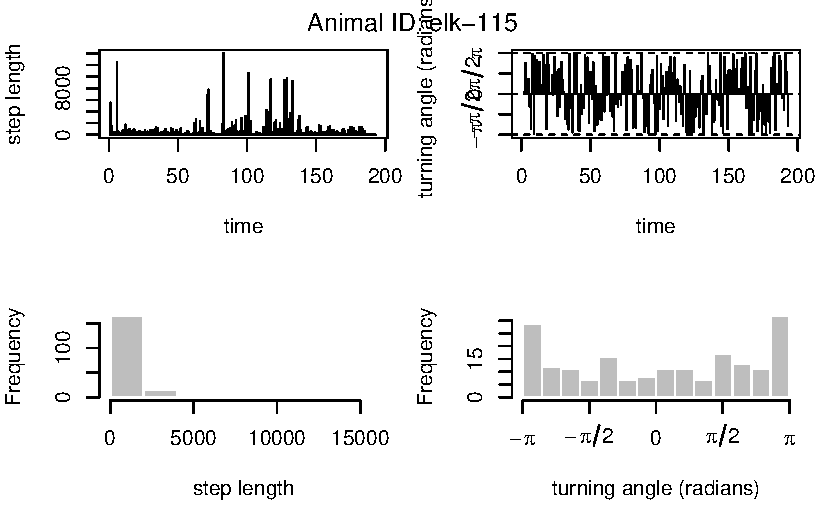
\includegraphics[keepaspectratio]{guide_files/figure-pdf/unnamed-chunk-2-2.pdf}}

\pandocbounded{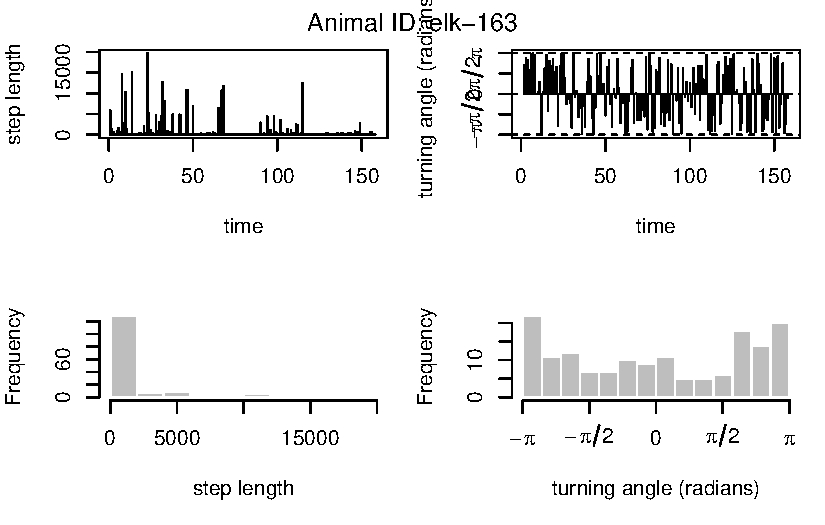
\includegraphics[keepaspectratio]{guide_files/figure-pdf/unnamed-chunk-2-3.pdf}}

\pandocbounded{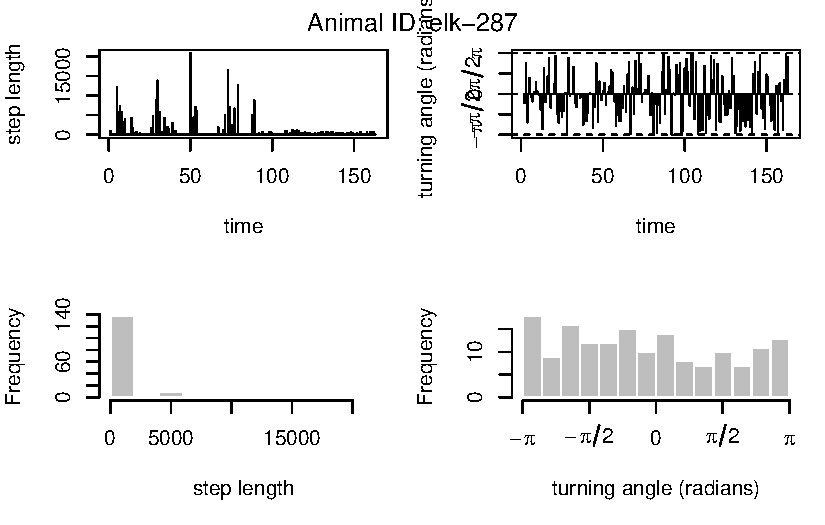
\includegraphics[keepaspectratio]{guide_files/figure-pdf/unnamed-chunk-2-4.pdf}}

\pandocbounded{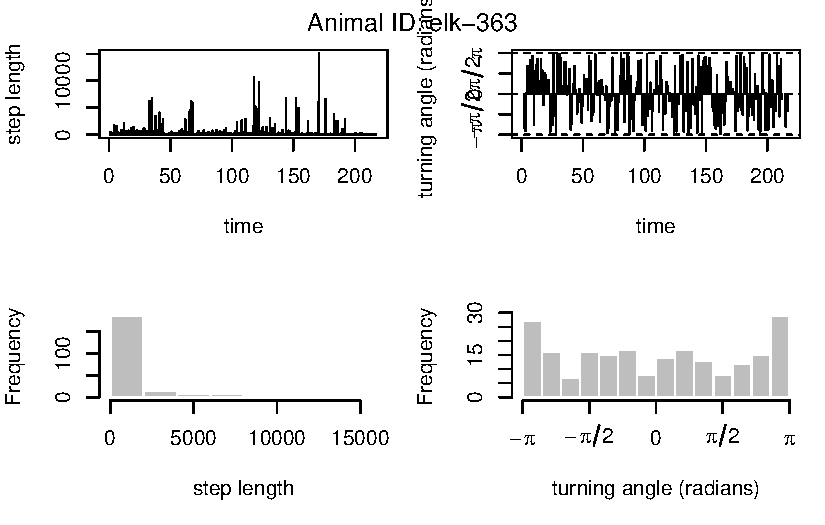
\includegraphics[keepaspectratio]{guide_files/figure-pdf/unnamed-chunk-2-5.pdf}}

\section{Fitting the Model}\label{fitting-the-model}

Next, choose the number of hidden states in the model. For example, a
basic model might include two states:

\begin{itemize}
\tightlist
\item
  Traveling
\item
  Foraging
\end{itemize}

It can then be fit using the \texttt{fitHMM()} function. The function
estimates the movement characteristics associated with each hidden state
and the probabilities of switching between states:

\begin{Shaded}
\begin{Highlighting}[]
\NormalTok{mu0 }\OtherTok{\textless{}{-}} \FunctionTok{c}\NormalTok{(}\DecValTok{50}\NormalTok{, }\DecValTok{300}\NormalTok{) }\CommentTok{\# step mean (two parameters: one for each state)}
\NormalTok{sigma0 }\OtherTok{\textless{}{-}} \FunctionTok{c}\NormalTok{(}\DecValTok{50}\NormalTok{,}\DecValTok{200}\NormalTok{) }\CommentTok{\# step SD}
\NormalTok{zeromass0 }\OtherTok{\textless{}{-}} \FunctionTok{c}\NormalTok{(}\FloatTok{0.1}\NormalTok{,}\FloatTok{0.01}\NormalTok{) }\CommentTok{\# step zero{-}mass}
\NormalTok{stepPar0 }\OtherTok{\textless{}{-}} \FunctionTok{c}\NormalTok{(mu0,sigma0,zeromass0)}

\NormalTok{angleMean0 }\OtherTok{\textless{}{-}} \FunctionTok{c}\NormalTok{(pi,}\DecValTok{0}\NormalTok{) }\CommentTok{\# angle mean}
\NormalTok{kappa0 }\OtherTok{\textless{}{-}} \FunctionTok{c}\NormalTok{(}\FloatTok{0.5}\NormalTok{,}\DecValTok{2}\NormalTok{) }\CommentTok{\# angle concentration}
\NormalTok{anglePar0 }\OtherTok{\textless{}{-}} \FunctionTok{c}\NormalTok{(angleMean0,kappa0)}

\NormalTok{model }\OtherTok{\textless{}{-}} \FunctionTok{fitHMM}\NormalTok{(}\AttributeTok{data=}\NormalTok{data,}\AttributeTok{nbStates=}\DecValTok{2}\NormalTok{,}\AttributeTok{stepPar0=}\NormalTok{stepPar0,}
\AttributeTok{anglePar0=}\NormalTok{anglePar0)}
\end{Highlighting}
\end{Shaded}

Notice we chose some initial parameters based on moveHMM's documentation
Theo Michelot, Langrock, and Patterson (2025).

\section{Interpreting the Results}\label{interpreting-the-results}

After fitting the model, the output will have estimates for the
parameters associated with each state and the probabilities of
transitioning between them.

We can also plot our model to view for a more straightforward summary of
our results:

\begin{Shaded}
\begin{Highlighting}[]
\FunctionTok{plot}\NormalTok{(model)}
\end{Highlighting}
\end{Shaded}

\begin{verbatim}
Decoding states sequence... DONE
\end{verbatim}

\pandocbounded{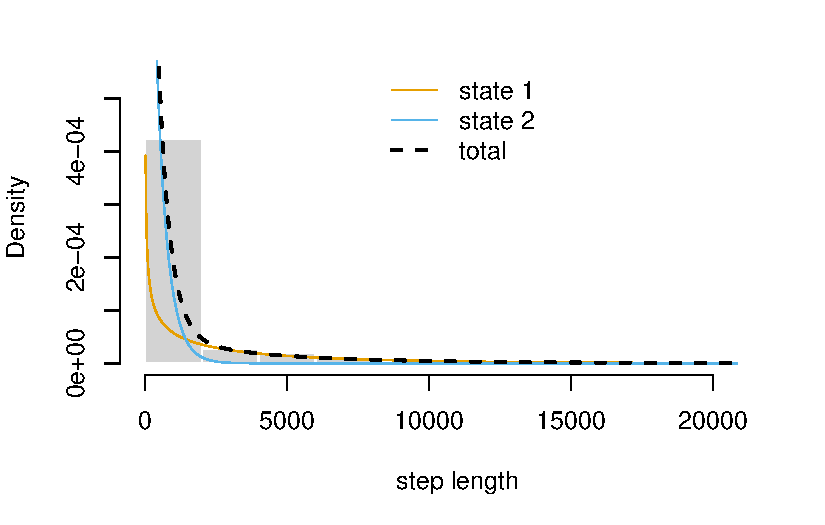
\includegraphics[keepaspectratio]{guide_files/figure-pdf/unnamed-chunk-4-1.pdf}}

\pandocbounded{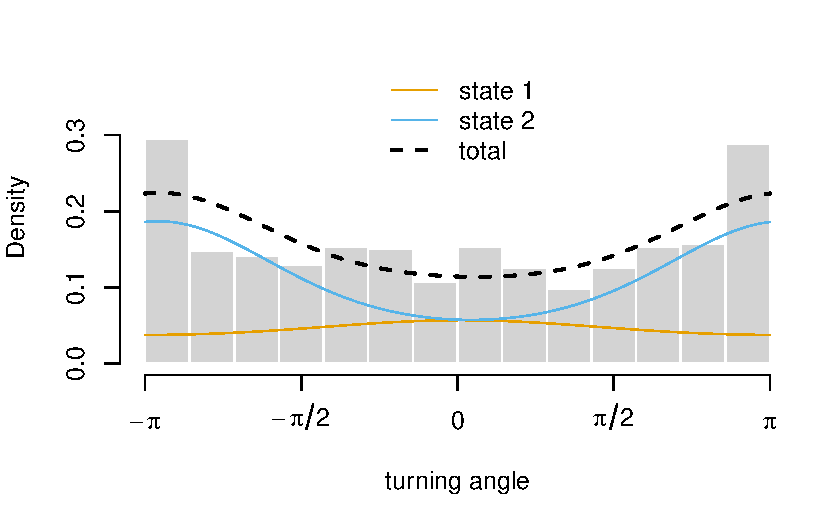
\includegraphics[keepaspectratio]{guide_files/figure-pdf/unnamed-chunk-4-2.pdf}}

\pandocbounded{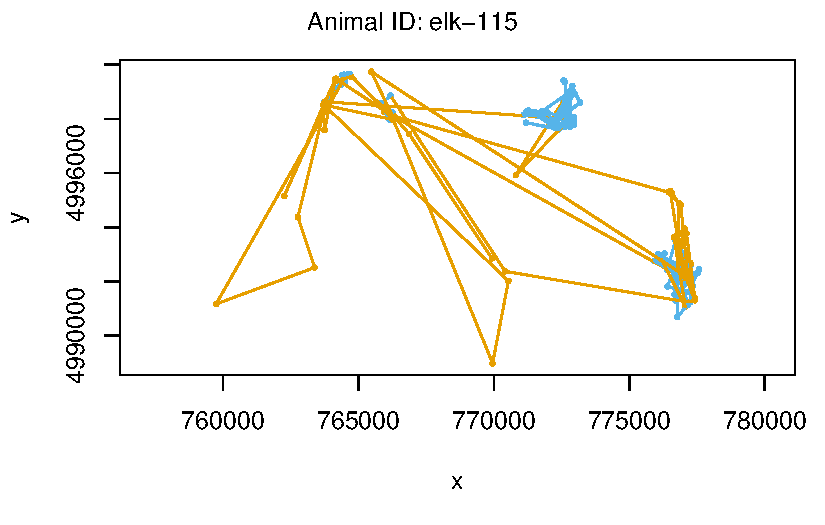
\includegraphics[keepaspectratio]{guide_files/figure-pdf/unnamed-chunk-4-3.pdf}}

\pandocbounded{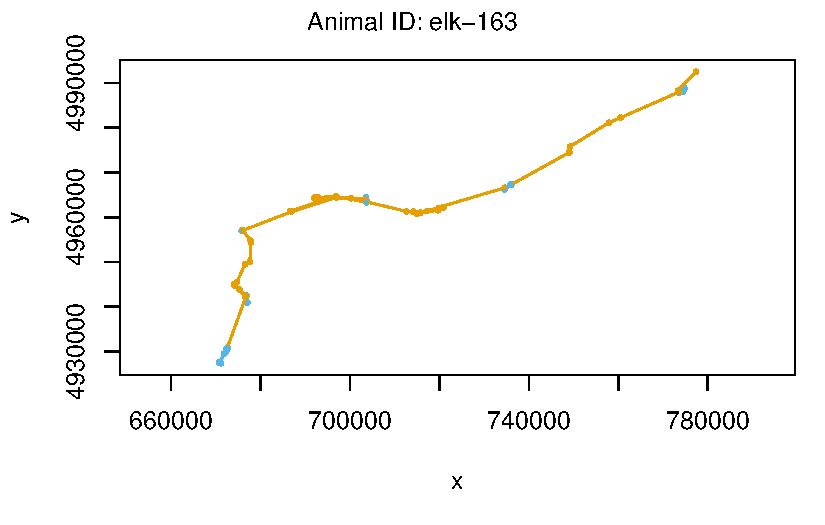
\includegraphics[keepaspectratio]{guide_files/figure-pdf/unnamed-chunk-4-4.pdf}}

\pandocbounded{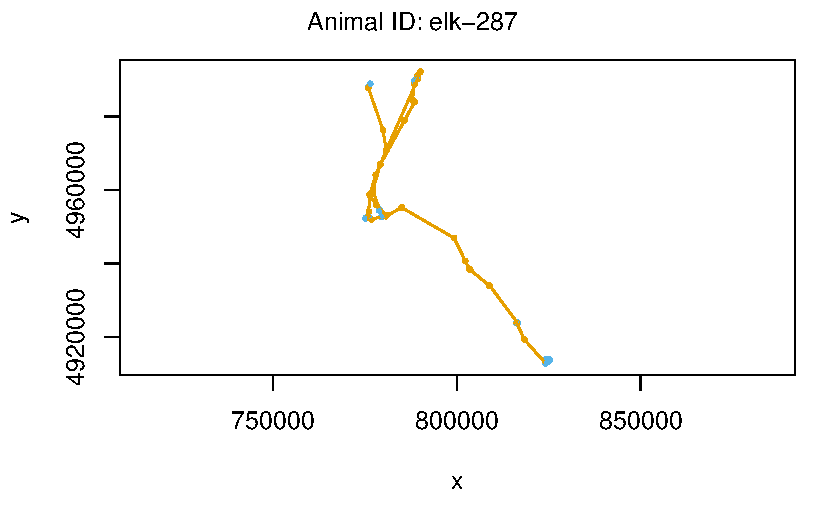
\includegraphics[keepaspectratio]{guide_files/figure-pdf/unnamed-chunk-4-5.pdf}}

\pandocbounded{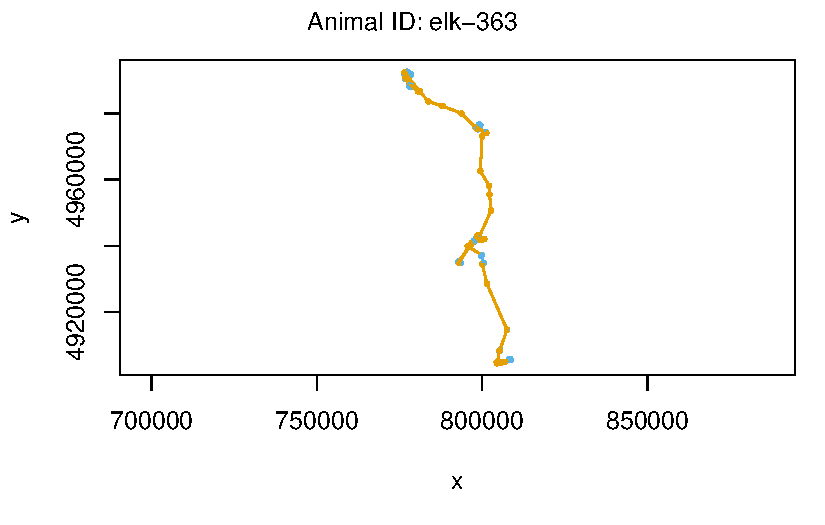
\includegraphics[keepaspectratio]{guide_files/figure-pdf/unnamed-chunk-4-6.pdf}}

The plots display the estimated step-length and turning-angle
distributions for each hidden state, along with the probabilities of
transitioning between states. These visualizations help identify
movement patterns associated with different behaviors.

Researchers can examine these results to interpret animal behavior. For
example, a state associated with longer step lengths and straighter
movement may represent traveling, while shorter step lengths and more
turning may be foraging.

\section{Limitations}\label{limitations}

The results of an HMM depend on assumptions such as the number of states
and the distributions used to model the data. Because of this, it is
important to check whether the chosen states make sense and to compare
alternative specifications if possible.

\bookmarksetup{startatroot}

\chapter*{References}\label{references}
\addcontentsline{toc}{chapter}{References}

\markboth{References}{References}

\phantomsection\label{refs}
\begin{CSLReferences}{1}{0}
\bibitem[\citeproctext]{ref-michelotMoveHMMPackageAnalysis}
Michelot, Theo, Roland Langrock, and Toby Patterson. 2025. {``{moveHMM}:
An {R} Package for the Analysis of Animal Movement Data,''} October.

\bibitem[\citeproctext]{ref-michelotMoveHMM2016}
Michelot, Théo, Roland Langrock, and Toby A. Patterson. 2016.
{``moveHMM: An r Package for the Statistical Modelling of Animal
Movement Data Using Hidden Markov Models.''} \emph{Methods in Ecology
and Evolution}.

\end{CSLReferences}

\cleardoublepage
\phantomsection
\addcontentsline{toc}{part}{Appendices}
\appendix

\chapter{Topic}\label{topic}

This user guide focuses on the use of hidden Markov models (HMMs) for
analyzing animal tracking data. HMMs are commonly used to predict
unobserved behaviors, like foraging, traveling, or resting, from
observed movement data.

The scope of this guide is limited to a conceptual overview of how HMMs
are applied to animal tracking data and how their outputs are
interpreted. It assumes basic knowledge in statistics and R, but won't
directly cover the mathematics and processes of HMMs.

\begin{tcolorbox}[enhanced jigsaw, colback=white, colbacktitle=quarto-callout-note-color!10!white, coltitle=black, opacitybacktitle=0.6, bottomrule=.15mm, colframe=quarto-callout-note-color-frame, toptitle=1mm, leftrule=.75mm, opacityback=0, bottomtitle=1mm, toprule=.15mm, rightrule=.15mm, titlerule=0mm, breakable, left=2mm, arc=.35mm, title=\textcolor{quarto-callout-note-color}{\faInfo}\hspace{0.5em}{Comments/suggestions}]

Ok, I think that's reasonable. You may want to find an R package that
allows you to fit such models without going into the math - it will
probably make your life easier to demonstrate how to do the input and
interpret the output if you have a specific package that will handle the
math details.

\end{tcolorbox}

\chapter{Needs Assessment}\label{needs-assessment}

What does someone trying to accomplish your chosen task need help with?

Someone trying to use HMMs for animal tracking data would probably need
a way to understand what HMMs and and how to apply them to R

What parts are likely to be tricky?

\begin{itemize}
\tightlist
\item
  Understanding hidden states
\item
  Choosing the amount of states
\item
  Interpreting the output
\item
  Preparing the movement data
\end{itemize}

What resources are already available on this topic that may be helpful?
Look for e.g.~software vignettes, package documentation, papers about
software packages, and so on.

\begin{itemize}
\tightlist
\item
  R package documentation like \texttt{moveHMM} or \texttt{momentuHMM}
\item
  Help files in R
\item
  Package vignettes
\end{itemize}

\begin{tcolorbox}[enhanced jigsaw, colback=white, colbacktitle=quarto-callout-note-color!10!white, coltitle=black, opacitybacktitle=0.6, bottomrule=.15mm, colframe=quarto-callout-note-color-frame, toptitle=1mm, leftrule=.75mm, opacityback=0, bottomtitle=1mm, toprule=.15mm, rightrule=.15mm, titlerule=0mm, breakable, left=2mm, arc=.35mm, title=\textcolor{quarto-callout-note-color}{\faInfo}\hspace{0.5em}{Note}]

I'd expect you to have read the vignettes and identified which ones are
helpful for each of the tricky parts.

\end{tcolorbox}

\chapter{Task Analysis}\label{task-analysis}

Here are some questions to guide you through the process of doing a task
analysis. You don't have to specifically answer each one of these (and
some may not apply), but they should get you started thinking in the
right direction.

What are the prerequisites, for both knowledge and e.g.~software setup?

\begin{itemize}
\tightlist
\item
  Knowledge of R
\item
  Installed HMM package
\item
  Animal tracking data
\end{itemize}

What are the basic requirements for any data that the method is used on?
- Generally no missing data - Should be ordered in time

\begin{tcolorbox}[enhanced jigsaw, colback=white, colbacktitle=quarto-callout-note-color!10!white, coltitle=black, opacitybacktitle=0.6, bottomrule=.15mm, colframe=quarto-callout-note-color-frame, toptitle=1mm, leftrule=.75mm, opacityback=0, bottomtitle=1mm, toprule=.15mm, rightrule=.15mm, titlerule=0mm, breakable, left=2mm, arc=.35mm, title=\textcolor{quarto-callout-note-color}{\faInfo}\hspace{0.5em}{Note}]

Ok, so what variables does animal tracking data have? Do you need
lat/long and time? In what format? What does animal tracking data look
like for the specific types of models you're considering?

\end{tcolorbox}

What are the basic components of the task?

\begin{enumerate}
\def\labelenumi{\arabic{enumi}.}
\tightlist
\item
  Import and clean tracking data\\
\item
  Calculate step lengths and turning angles\\
\item
  Choose the number of hidden states\\
\item
  Fit the HMM\\
\item
  Interpret state estimates and transition probabilities
\end{enumerate}

What decisions does the user need to be prepared to make on the fly?

\begin{itemize}
\tightlist
\item
  How many hidden states to use
\item
  Whether the results make biological sense
\end{itemize}

What questions should the user ask of the ``first draft'' of the
product? What adjustments may need to be made?

\begin{itemize}
\tightlist
\item
  Did the model converge?
\item
  Do the states correspond to realistic behaviors?
\item
  Would a different number of states improve the model?
\end{itemize}

\section{Additional Guidance}\label{additional-guidance}

Your check-in should answer these basic questions (and similar concerns
that apply more directly to your topic).

Once you've completed the check-in, you can use this section to
jump-start an introduction/set-up/getting started section in your user
guide. This document should remain as an appendix to your main report.




\end{document}
